\section{Transformations}
\label{sec:transformations}

We follow the IR step by step as it is transformed, considering a \lstinline|linalg.conv_1d_nwc_wcf| operation and its lowering to a tiled, padded and vectorized form.
The input IR is shown in Figure~\ref{fig:lifecycle_tiling} (left).

\begin{figure}[h!tb]
    \noindent
    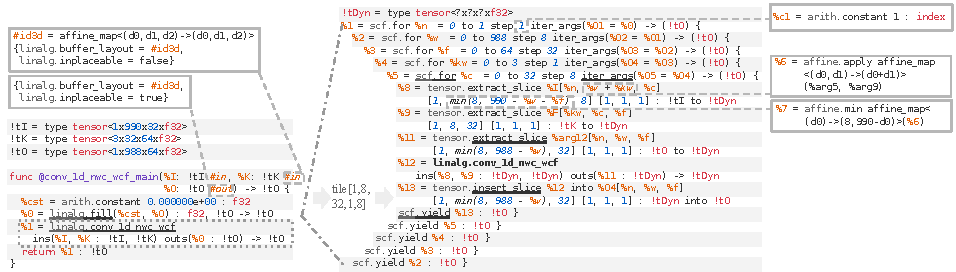
\includegraphics[width=\textwidth]{figures/tiling}
    \caption{Tiling a convolution on tensors introduces loops with secondary induction variables, pseudo-IR. Parts in italic are simplified for clarity and expanded in callouts. Underscored parts refer to new concepts: (left) operations on immutable tensors, (right) secondary induction variables and tensor slicing.}
    \label{fig:lifecycle_tiling}
\end{figure}

This level of abstraction operates on immutable SSA values: new tensor values are created from existing ones.
Memory locations only occur as annotations at function boundary to
specify how these tensors will materialize into memory, in a subsequent lowering step (more on this later).

The index notation corresponding to \lstinline|linalg.conv_1d_nwc_wcf|
is given by a $5$-D rectangular iteration domain operating on $3$-D tensors along with the expression:\footnote{The operation also allows specifying static sizes and strides that we omit here for simplicity}
\begin{equation*}
O[n,w,f] = I[n,w+k_w,c] . K[k_w,c,f]
\end{equation*}
The iteration domain is implicit in the operation description and is such that the iterators span the entire data of the operands. 
In this example, this is given by the inequalities 
$$
0\le n<O.0, \quad 0\le w<O.1, \quad 0\le f<O.2, \quad 0\le k_w<K.0, \quad 0\le c<K.1
$$
where $O.d$ denotes the size of the $d$-th dimension of $O$.
The derivation for these quantities follows the same rules as Tensor Comprehensions~\cite{vasilache2019next}. 
In the dense case, they can be derived with successive applications of the Fourier-Motzkin elimination procedure~\cite{schrijver86}. 

\subsection{Tiling}

Tiling the operation introduces \lstinline|scf.for| loops as well as subset operations (\lstinline|tensor.extract_slice| and \lstinline|tensor.insert_slice|) to access the tiled data Figure~\ref{fig:lifecycle_tiling} (right).
The tiled form of the operation is itself a \lstinline|linalg.conv_1d_nwc_wcf| operating on the tiled subsets.
The derivation of dense subsets is obtained by computing the image of the iteration domain by the indexing function for each tensor.
Non-dense iteration domains and subsets require IR extensions and inspector-executor~\cite{kjolstad2017taco}
code generation that are outside the scope of this paper.

Back to our example, we chose tile sizes of \lstinline|1x8x32x1x8|.
While these sizes are static, some divisions are not integral and the boundary tiles are subject to full/partial tile classification.
As a result, there is no \emph{single static tensor type} that is valid for every loop iteration; the tiled tensor type \lstinline|!tDyn| must be relaxed to a
dynamically shaped tensor.\footnote{Note that our compilation flow supports full dynamism, although for illustration purposes we focus on static inputs.}.
The dynamic tile sizes needed to access the tile data slices are \%8, \%9 and \%11.
Separate canonicalizations later kick in to further refine the types that can be determined to be partially static.

The \lstinline|scf.for| loops introduced by this ``tiling on tensors'' transformation 
perform iterative yields of the full tensor value that is produced at each iteration of
the loop nest. The yielding form of \lstinline|scf.for| combined with subset operations 
generalize the insertion into a structure to a more dynamic type (see Section~\ref{subsubsec:tensor-dialect}).
Since tensor values are immutable, new values are produced by each \lstinline|tensor.insert_slice| and \lstinline|scf.yield|. 
It is the responsibility of the bufferization process to avoid superfluous
allocations and copies.

\subsection{Padding Values and Packing}
\label{subsec:padding-values-and-packing}

When tiling is applied, the content of a tile can often become more dynamic to account for boundary effects.
This hampers vectorization which requires static sizes.
There are multiple mitigating options:
\begin{enumerate}
    \item Tiling may trigger multi-level loop peeling (or versioning) to isolate the statically known constant part of the problem in a main loop, followed by cleanup loops for the boundaries. 
    The cleanup loops still exhibit dynamic behavior but they can always be tiled by $1$ and
    further reduce to a dimension of size $1$ that can be vectorized in a finer-grained form.
    \item An alternative is to pad the dynamic tile to a larger known static size.
    The value used for padding must be the neutral for the consuming operation.
    This introduces extra copies and more computations at the boundary but all tiles now become full.
    \item A third alternative is to turn to a representation that involves explicit masking.
    This is work in progress and outside the scope of this paper.
\end{enumerate}

\begin{figure}[h!tb]
    \noindent
    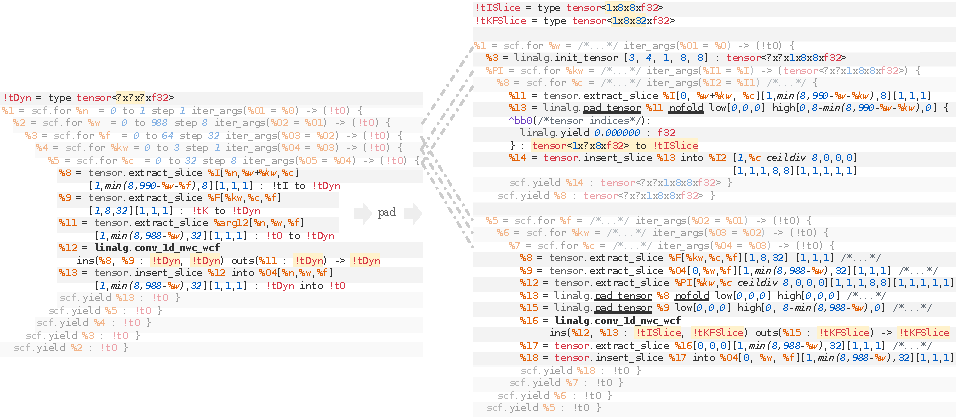
\includegraphics[width=\textwidth]{figures/padding}
    \caption{Padding a tiled operation to obtain fixed-size tensors (highlighted), pseudo-IR. Parts in italic are simplified for brevity. Constants in roman font are attributes, in italic are \texttt{arith.constant} operation results. The \texttt{nofold} padding persists in the IR even without type change and may be later placed in a fast buffer. Trailing type annotations sometimes omitted for brevity.}
    \label{fig:lifecycle_padding}
\end{figure}

When the computation does not entail enough temporal locality, peeling is almost always the 
better choice.
As soon as some temporal locality is available, the copy required for padding can be amortized.
Padding then also serves the purpose of aligning memory accesses in the padded buffer, once bufferization has occurred.
This is particularly important to avoid \emph{cache line splitting}, i.e., partially clobbering cache lines and inducing extraneous data transfers through the cache hierarchy; it is often required to reach the highest levels of performance.
In other words, value padding also implies address padding.\footnote{Additional masking may in turn facilitate address padding.}

Padding is materialized by the introduction of \lstinline{tensor.pad} operations, and its size is obtained by subtracting the dynamic tile size from the static tile size. 
All elements in the padded region are set to the constant value \lstinline[mathescape]!%cst!. 
This makes all operands of the tiled convolution statically shaped.

When the tile shape is already known to be static, value padding is not required for vectorization. In such cases, \lstinline|linalg.pad| would
simply fold away.
We additionally support a \emph{nofold} attribute to force padding to 
occur in such cases where address alignment is essential to avoid cache line split.

Operations that exhibit temporal reuse of the data may additionally
benefit from hoisting the padding operation out of the tile loops and storing the padded tiles in a higher-dimensional packed tensor. This allows both
amortizing the cost of copying as well as physically laying out tiles
contiguously in an intermediate buffer. This results in a smaller distance in memory between tiles that are reused within a short time-span
and reduces TLB misses.

The amount of hoisting is configurable per tensor and exhibits various
trade-offs between memory consumption, cost of copy and benefits to the 
computation primitive.

In the example of Figure~\ref{fig:lifecycle_padding}, the input tensor padding is hoisted by $3$ loops. 
This introduces an additional tile loop nest to precompute the padded tiles and insert them into the packed tensor of type \lstinline|tensor<?x?x1x8x8xf32>| containing all padded tiles.
Inside the original tile loop nest, the padding is replaced by an access to the packed tensor \lstinline|%12= tensor.extract_slice %PI...|.

Similarly to the tiling case, the sizes of packed tensor are obtained by computing the image of the iteration domain by a function of the enclosing loop variables and the tensor's indexing function.

\subsection{Vectorization}
\label{subsec:vectorization}

After tiling and padding, the convolution operands are statically shaped and are in a good state for vectorization, see Figure~\ref{fig:lifecycle_vectorization} (left).
In the current IR, only $2$ types of operations need to be
vectorized: \lstinline|tensor.pad| and 
\lstinline|linalg.conv1d_nwc_wcf|.

\begin{figure}[h!tb]
    \noindent
    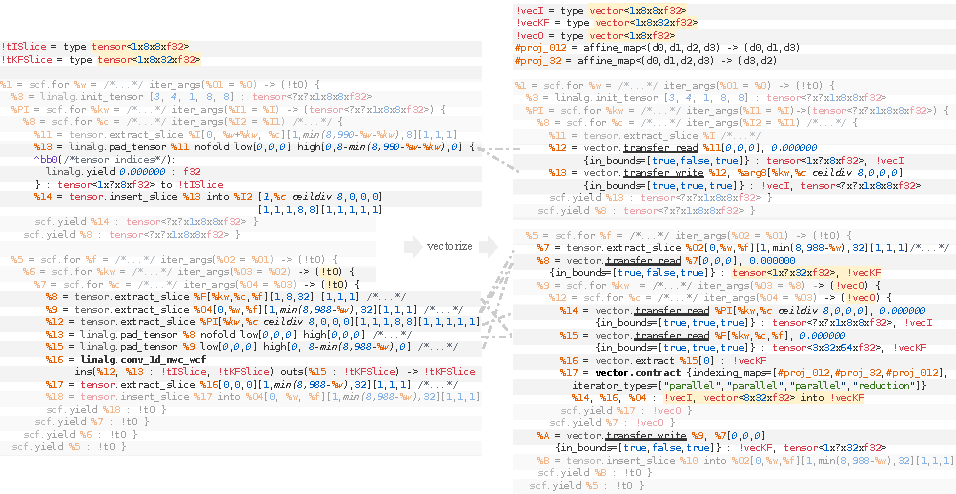
\includegraphics[width=\textwidth]{figures/vectorization}
    \caption{Operations on tensors of fixed sizes can be directly vectorized, pseudo-IR. Parts in italic are simplified for brevity as in Figure~\ref{fig:lifecycle_padding}. Vector values are immutable. They can be read from and written into tensors. Out-of-bounds access is allowed; reads replicate the scalar operand, writes are ignored.}
    \label{fig:lifecycle_vectorization}
\end{figure}

The vectorization of \lstinline|tensor.pad| is implemented with a simple one-off pattern that reduces it to a pair of \lstinline|vector.transfer_read|, \lstinline|vector.transfer_write| operations. 
The \lstinline{vector.transfer} operations are often referred to as a \emph{Swiss army knife} for bridging the gap between memory and vectors. 
In particular, they carry enough information to encode various multi-dimensional vector memory read and write patterns (e.g., broadcasted, permuted, masked, padded accesses).
They can be easily retargeted to specifics of current and future memory subsystems and vector ISAs.
With the existence of such an operation, the vectorization of 
\lstinline|tensor.pad| is comparatively a very small and progressive lowering step.\footnote{Especially if one thinks about all the load, store, indexing and fill operations that result from such a construct.}
The vector dialect additionally provides a first-class representation for high-intensity operations.
These operations are a key building block for high-performance codegen.
Figure~\ref{fig:lifecycle_vectorization} (right) illustrates one such operation, \lstinline{vector.contract}, in action.

The vectorization of \lstinline|linalg| operations follows a recipe that introduces a \lstinline{vector.transfer_read} for each operand, performs the computation in vector form and commits it back to the proper tensor or buffer via a \lstinline{vector.transfer_write}.
The \lstinline{vector.transfer} operations are indexed following the indexing expressions of the 
\lstinline|linalg| operation.
This behavior is generic for the data movement part of all \lstinline|linalg| operations.

The vectorization of the computation part is subject to variations.
Under the hood, every \lstinline|linalg| operation has a body region that expresses the scalar form of
the computation \footnote{The body may be printed explicitly (when expressed in \lstinline|linalg.generic| form)
or simply elided when expressed in "named" form (such as \lstinline|linalg.conv_xxx|).}.
The body vectorization depends on the type of indexings the parent \lstinline|linalg.generic| performs:
\begin{enumerate}
\item In the simplest case of pointwise operations (indexings are all identity), every operation in the body is simply written as a pointwise vector variant.
\item Lower dimensional tensor operands can be \lstinline|vector.broadcast| into higher-dimensional vectors where needed and reduce to the previous case.
\item Permutations in indexing expressions are handled with \lstinline|vector.transpose| operations.
\item Reduction dimensions lower to a first-class \lstinline{vector.contract} or \lstinline{vector.multi_reduction} depending on further analysis of the body.
\item Sliding window patterns such as convolutions are handled specially by unrolling along 
certain dimensions and extracting slices that further reduce to \lstinline{vector.contract} or
\lstinline{vector.fma}. This simple strategy delivers high performance
while capturing strided and dilated convolutions.
\end{enumerate}

In our running example of Figure~\ref{fig:lifecycle_vectorization} (right), the dimension corresponding to the \lstinline|%kw| loop would be unrolled. For the purpose of this illustration we have used a 
tile size of $1$ which does not further unroll. Note the 
\lstinline|%16 = vector.extract %15[0] : !vecK| operation which is a degenerate form of unrolled slice
extraction for size $1$.
Additional canonicalization and folding patterns occur that simplify chains of \lstinline|vector.transfer| operations, as well as move loop-independent instructions out of loops
(e.g.\ \lstinline|%8 = vector.transfer_read|).
Also note that the loops \lstinline|%9 = scf.for ...| and \lstinline|%12 = scf.for ...| both
yield vector values without inserting or extracting from a tensor.
This will guarantee no roundtrip to memory after bufferization.

All these transformations are implemented by following SSA def-use chains and legal by design (see Section~\ref{subsec:discussion} for a discussion of this principle).

\subsection{Bufferization}
\label{subsec:tensor-bufferization}

Bufferization is the process of materializing \texttt{tensor} values into memory (\texttt{memref}). 
It is necessary to make tensor programs concretely executable with a source
of data residing in memory.
In our current compilation pipeline, it is one of the last steps.

Tensors in \MLIR are immutable. An operation that produces a new tensor value (maybe from another input tensor) is conceptually an entirely new tensor. Unlike with \texttt{memref}s, there is no concept of updating/writing to a tensor in-place. To achieve good performance, it is essential to:

\begin{itemize}
    \item Allocate as little memory as possible.
    \item Copy as little memory as possible.
\end{itemize}

Buffers should be reused and updated in-place whenever possible or risk large performance penalty when program transformations result in unexpected allocation and copying.

\begin{figure}[h!tb]
    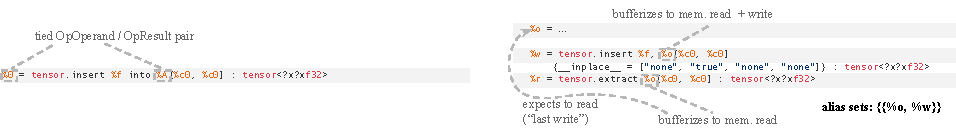
\includegraphics[width=\textwidth]{figures/bufferization_notation_conflict}
    \caption{Left-hand side: output tensor arguments, tied with the result of an operation, in destination-passing style. Right-hand side: example of a read-after-write conflict.}
    \label{fig:bufferization_notation_conflict}
\end{figure}

\paragraph{Read-after-Write Conflicts}
Allocating a new buffer for every memory write is always safe, but wastes memory and introduces unnecessary copies. 
On the other hand, reusing a buffer and writing to it in-place can result in invalid bufferization if the original data at the overwritten memory location must be read at a later point of time. 
When performing transformations, one must be careful to preserve program semantics exposed by dependencies~\cite{AllenKennedy}.
The right-hand side of Figure~\ref{fig:bufferization_notation_conflict} illustrates a potential \emph{Read-after-Write (RaW) conflict} that prevents in-place bufferization. 
The problem of efficient bufferization is related to register coalescing, the register allocation sub-task associated with the elimination of register-to-register moves.

\paragraph{Destination-Passing Style}
The current heuristic we are offering for bufferization is well-suited for operations that are in \emph{destination-passing style}. 
In such operations, one of the tensor arguments is tied with the resulting tensor for in-place bufferization.
Such a tensor argument is called an \emph{output} tensor, see the left-hand side of Figure~\ref{fig:bufferization_notation_conflict}. 
Intuitively, output tensors are similar to C++ \emph{output parameters} that are passed as non-const references and used for returning the result of a computation. 
Except these ties between an output tensor (argument) and the operation's result serve as a bufferization constraint with no observable impact on the functional semantics; in particular, output tensors still appear as immutable.
During bufferization, only output tensors are considered when looking for a buffer to write the result of an operation into.

The rationale derives \emph{from first principles} when composing structured operations with \lstinline{scf.for}, the natural target for lowering multidimensional tensor operations.
Since \lstinline{scf.for} yields a value as a result, its nested region must yield fully defined tensors rather than arbitrary subsets.
Since nested operations typically apply to tensor subsets --- often resulting from \lstinline{linalg} tiling transformations --- a pair of matching \lstinline{extract_slice}/\lstinline{insert_slice} operations are typically injected.
These, and the associated \lstinline{scf.yield} operation, naturally consume their tensor argument (i.e., there cannot be any subsequent uses of it), which makes them ideal candidates for in-place bufferization. 
A comprehensive example is shown in Figure~\ref{fig:lifecycle_bufferization}.

This heuristic design appears to work well on the kind of IR we are dealing with when operating on the \texttt{linalg} dialect:
\begin{itemize}
    \item We saw that tiling produces outer loops iterating on tiled subsets. Operations to manage these subsets, such as \lstinline{extract_slice}, \lstinline{insert_slice}, are naturally in destination-passing style.
    \item Padding, packing, vectorization, and other transformations also produce operations with a destination-passing style semantics, on full tensors or subsets.
    \item \lstinline{linalg.generic} itself is designed as a destination-passing style operation. This includes \lstinline{linalg.matmul} and any other operation that reduces to \lstinline{linalg.generic}.
\end{itemize}

\begin{figure}[h!tb]
    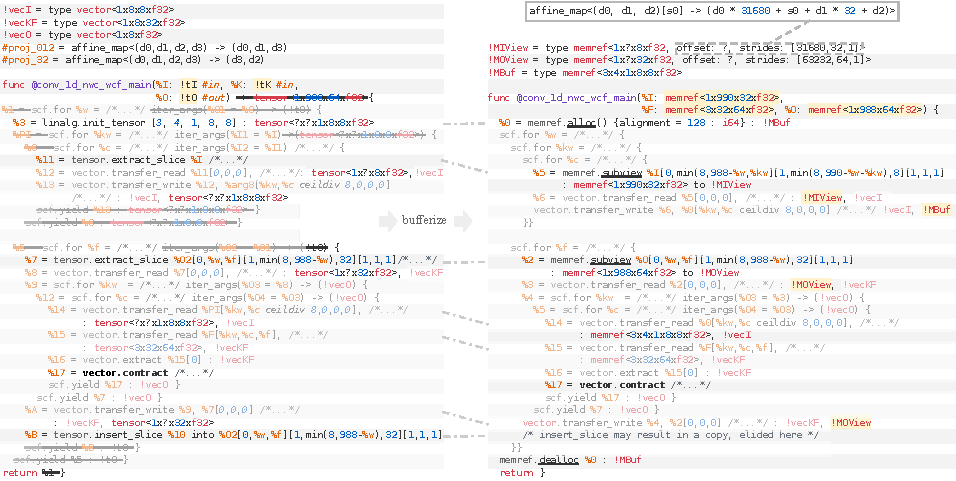
\includegraphics[width=\textwidth]{figures/bufferization}
    \caption{Bufferization assigns tensor values to buffers, taking into account function-level annotations \texttt{\#in}, \texttt{\#out} from Figure~\ref{fig:lifecycle_tiling}. Data flow is replaced by side effects, unnecessary values are crossed out on the left. Temporary buffers may be allocated to ensure contiguous access patterns. ``Computational payload'' dialects such as \texttt{linalg} and \texttt{vector} are designed to support both \texttt{tensor} and \texttt{memref} (buffer) containers.}
    \label{fig:lifecycle_bufferization}
\end{figure}

To illustrate this rationale, consider \texttt{tensor.insert} as an example of an operation in destination-passing style. 
A tensor result of an operation may have one or multiple \emph{potentially aliasing OpOperands} in the bufferization framework. 
For example, the only potentially aliasing OpOperand of \texttt{\%0} in the example is \texttt{\%A} (Figure~\ref{fig:bufferization_notation_conflict}, left-hand side), meaning that after bufferization:
\begin{itemize}
    \item \emph{buffer(}\texttt{\%0}\emph{)} = \emph{buffer(}\texttt{\%A}\emph{)}
    \item Or: \emph{buffer(}\texttt{\%0}\emph{)} is a newly allocated buffer.
\end{itemize}
No other operands are taken into account when choosing a buffer. 
Operations that do not have a potentially aliasing OpOperand for their tensor results always allocate a new buffer. 
For example, \texttt{tensor.generate} always allocates after bufferization.

This bufferization design is a heuristic: operations with no natural candidate output tensor (e.g.\ the sum of two tensors) allocate and copy by default.
This simplifies the bufferization problem, reducing it to an analysis of use-def chains.
The tradeoff is that upstream compilation passes are responsible of rewriting the IR in destination-passing style.
We believe a global copy elimination problem could be formalized on top of destination-passing style, offering the best of both worlds in terms of allowing passes to optimize bufferization at a global scale, while still enabling a robust, in-place bufferization path for the important special case of refining structured operations.

\paragraph{Analysis of Tensor SSA Use-Def Chains}
During bufferization, each operation with tensor semantics is replaced with an operation with memref semantics. 
Before modifying any IR, an analysis decides for each tensor OpOperand \texttt{\%t} whether \emph{buffer(}\texttt{\%t}\emph{)} (\emph{in-place bufferization}) or a copy thereof (\emph{out-of-place bufferization}), denoted by \emph{copy(buffer(}\texttt{\%t}\emph{))}, should be used with the new memref operation. 
The analysis simulates \emph{a future in-place bufferization of the OpOperand} and checks if a RaW conflict can be found under this assumption. 
If not, the analysis greedily commits to this in-place bufferization decision. 
Furthermore, the analysis stores the fact that the OpOperand and its potentially aliasing OpResult are now \emph{known to alias}, by merging their alias sets.

The search for RaW conflicts is based on a traversal of tensor SSA use-def chains. 
When simulating the in-place bufferization of an OpOperand \texttt{\%o}, the analysis looks for all uses of this SSA value (and its aliases) that bufferize to a memory read.
For each read, it walks the IR back the \emph{last write} of the tensor; i.e., the value that defines the contents of the tensor (skipping over operation like \texttt{tensor.cast} or \texttt{tensor.extract\_slice} that do not bufferize to a memory write). 
This is the value that the operation is expected to read. 
If an interleaved ``future write'' of an aliasing buffer exists, then there would be a RaW conflict.

The in-place bufferization of \texttt{\%o} of the \texttt{tensor.insert} (Figure~\ref{fig:bufferization_notation_conflict}, right-hand side) is a RaW conflict (and would thus be an invalid bufferization) because the operation is in-between the definition of \texttt{\%o} and the \texttt{tensor.extract} operation, which is expected to read the original value of \texttt{\%o} and not \texttt{\%w}.

\paragraph{Extension Points}
The bufferization framework is customizable and can be adapted for different use cases via two main extension mechanisms.

First, the order in which operations are analyzed is a heuristic and affects the order in which RaW conflicts are detected. 
There are often multiple out-of-place bufferization candidates that can prevent a RaW conflict. 
Only when a RaW conflict is no longer avoidable, the analysis decides to bufferize an OpOperand out-of-place. Therefore, operations (and their OpOperands) that are analyzed earlier are less likely to bufferize out-of-place. By analyzing a certain group of operations first, the analysis can be steered towards bufferizing these operations in-place and trying to avoid RaW conflicts by bufferizing other operations out-of-place.

Second, operations can refine the analysis by specifying conidtions that should not be treated as RaW conflicts. 
For example, a \texttt{tensor.insert\_slice} operation only affect a subset of the entire buffer. 
This informatio can be used to make better bufferization decisions around matching \texttt{tensor.extract\_slice}/\texttt{tensor.insert\_slice} pairs.
This paves the way for more advanced analyses based on intersection and difference, as well as partial reuse, of buffer regions.

\subsection{Progressive Lowering of Multidimensional Vector Operations Towards LLVM}
\label{subsec:rewrites-and-foldings}

\begin{figure}[h!tb]
    \noindent
    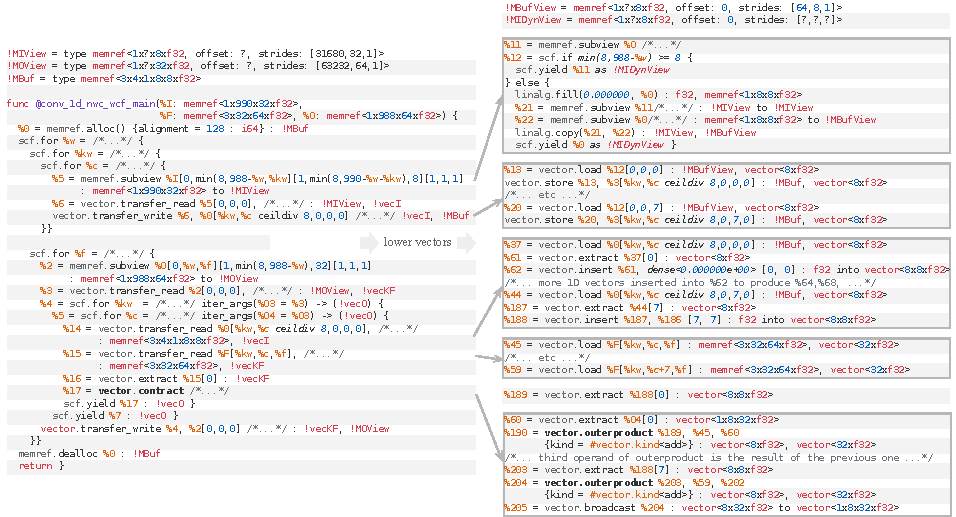
\includegraphics[width=\textwidth]{figures/lower_vectors}
    \caption{The \texttt{vector} dialect can be lowered progressively to simpler operations on 1-D vectors. Illustrated on lowering contractions to outer products, with parts in italic simplified for brevity and repetitive parts omitted. Lower-level vector operations require constant indices and are produced by unrolling the outer dimensions.}
    \label{fig:lifecycle_lower_vectors}
\end{figure}

At this time, the IR has reached a level of abstraction consisting of loops around buffers containing
multi-dimensional vectors and operations on those. This is now close to the C + vectors paradigm of
LLVM, with the exception that we operate on multi-dimensional vectors, whereas LLVM only has 1-D vectors.

In the simplest case, multi-dimensional \lstinline|vector.transfer| operations lower to multiple $1$-D \lstinline|vector.load| and \lstinline|vector.store| operations.
When supported by hardware, they can also lower to n-D DMA operations.
In more complex cases, transfer operations lower to a combination of broadcasts, tranpositions and masked scatter/gather.
In the particular case where the \lstinline|vector.transfer| cannot be determined to be in-bounds, 
one must resort to an additional separation between full and partial transfer, akin to the full and 
partial tile separation at the tile level.
This is illustrated in Figure~\ref{fig:lifecycle_lower_vectors} (right) in the \lstinline|else| block
around the \lstinline|linalg.copy(%21, %22)| operation.

\begin{figure}[h!tb]
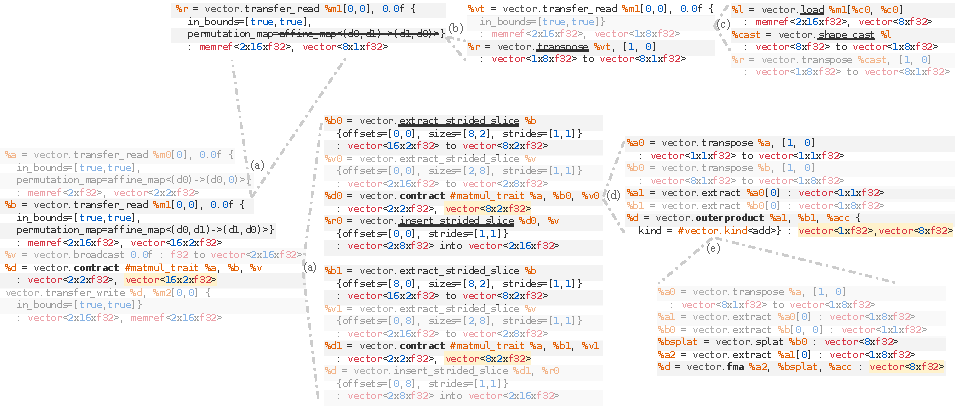
\includegraphics[width=\textwidth]{figures/vector_deeper}
\caption{Progressive lowering of the \texttt{vector} dialect operations representing matrix product: (a) vector unrolling with target shape $2\times8\times2$ introduces vector slice manipulation; (b) the transfer permutation is materialized as a \texttt{transpose} operation; (c) 1-D transfers become plain loads with shape adaptation; (d) contractions rewrite as outer products (other options are possible), which in turn lower to (e) fused multiply-add instructions.}
\label{fig:vector_deeper}
\end{figure}

Our pervasive use of n-D vector types effectively shielded an "unroll-and-jammed vector form", known to be efficient on vector hardware, from intermediate compilation phases that could interfere with later vectorization. At this point, this form is ready for progressive lowering into 1-D operations with almost 1-1 mapping to LLVM IR.

Let us illustrate the progressive lowering of operations on n-D vectors to lower-dimensional equivalents closer to hardware instructions. Starting from the vectorized matrix product code on the left of the Figure~\ref{fig:vector_deeper}. This IR is (mostly) retargetable since it is using higher-level \lstinline{transfer} and \lstinline{contract} operations that do not usually correspond to the available hardware instructions.\footnote{Even with \texttt{transfer} operations, vector sizes become hardware-specific and other aspects such as special ISA dimensions and the number of available registers come into play, but the representation is still easy to transform.} We first apply vector ``unrolling'' as in Figure~\ref{fig:vector_deeper}(a). The goal of this transformation is twofold: (1) it breaks down vector operations to sizes known to be well supported by the target, e.g., mapping to AMX instructions, and (2) preemtively handling non-power of $2$ sizes into power of $2$ compositions, e.g., \lstinline{vector<12xf32>} into 3 \lstinline{vector<4xf32>} to avoid suboptimal backend code generation~\cite{OuterproductSpilling}. The resulting IR is still partially retargetable as \lstinline{transfer} and \lstinline{contract} operations are still present and need to be lowered to a closer-to-hardware representation using one of the available schemes.

After unrolling, \lstinline|vector.extract_strided_slice| and \lstinline|vector.insert_strided_slice| extract and insert
slices of a vector into a larger vector. 
They are conceptually the same as their \lstinline{tensor} dialect counterparts.
When unrolling operations folding patterns can lead to insert and extract operations cancelling each other if the target shapes match.
Other peephole optimization patterns, applied along with the unrolling transformation,
track subsets through broadcast and transpose operations, all the way to transfer operations
where the may fold into memory reindexings.

Higher-level \lstinline|vector.transfer_read| usually cannot be directly lowered to a load instructions and are handled progressively:
first, by materializing transpositions as in Figure~\ref{fig:vector_deeper}(b), then, by creating 1-D loads and broadcasts as in Figure~\ref{fig:vector_deeper}(c).
Transpositions can in turn be implemented elementwise, with LLVM's \lstinline{shuffle} instruction or using dedicated intrinsics, depending on the configuration.

Similarly, \lstinline|vector.contract| can be lowered to outer products, inner (dot) products or LLVM IR matrix intrinsics.
In this example, it is lowered to outer products in Figure~\ref{fig:vector_deeper}(d)
to enable further mapping to SIMD fused multiply-add instructions in Figure~\ref{fig:vector_deeper}(e).
Each stage of the progressive lowering is accompanied by foldings and peephole optimizations that reduce the amount of IR to handle and enable additional transformations.
As the result, the fully lowered vector IR operates on \lstinline{vector<8xf32>}, supported for example by AVX2, and is quite compact. The resulting code for our example has several dozen operations and is provided in Appendix~\ref{sec:appendix-lowered-vector}. These operations are now ready for lowering to the LLVM dialect and further translation to LLVM IR.

\subsection{Discussion}
\label{subsec:discussion}

The levels of IR we introduced allow for developing an expressive set of essential transformations. These transformations are legal by design, in the sense that their legality and applicability derive from the operation's properties and structure.
We refer to this philosophy as \emph{transformations-oriented IR design}. 

\subsubsection{Transformation-Oriented IR Design}
\label{subsubsec:transformation-oriented-ir-design}

Traditional compiler analyses and transformations for numerical computing~\cite{AllenKennedy} revolve around trade-offs and questions related to:
\begin{itemize}
\item Legality, i.e.\ what transformations can be applied without changing the observed program semantics?
Legality conditions are often checked through static analyses. They may be performed upfront or on-demand, and their results may be updated as the IR is transformed.  
For example, dominance analysis produces necessary conditions for code motion: uses should remain dominated by definitions.
\item Applicability, i.e.\ how complex is the IR matching process for finding the place where to apply a transformation? How complex does the IR become after applying the transformation?
Applicability also encompasses considerations related to how much information has potentially been lost, whether the IR remains analyzable and whether subsequent transformations continue to be easily applicable.
\item Profitability, i.e.\ what are the transformations deemed beneficial for a given metric?
Profitability is often determined by heuristics or performance models. For example, polyhedral compilers often focus on finding an objective function to minimize (universal or target-specific) \cite{vasilache2019next}, while auto-tuners may rely on a learned performance model to accelerate search \cite{zheng2020ansor}.
\end{itemize}

It is of central importance to control the abstractions on which the transformation legality, applicability and  profitability questions relate to.
The finer-grained the IR, the more general and canonical the representation, but also the more intractable the analyses and transformations.
Indeed, canonicalization to some flavor of \LLVM IR consisting of a Static Single Assignment (SSA) form Control Flow Graph (CFG) has proven invaluable in enabling the reuse of common infrastructure for middle-end and back-end compilers.
But lowering abstractions and domain knowledge too quickly reduces the amount of structure available to derive transformations from.
While manipulating loops is a net gain compared to control flow graphs for a certain class of transformations, important information is still lost (e.g.\ parallel and reduction multi-loop semantics, loop-level data flow and memory footprint, substitution of a full loop nest with an external implementation).
It induces non-trivial phase ordering issues: loop fusion to enhance temporal locality may alter the ability to recognize an efficient BLAS-2 or BLAS-3 implementation in a numerical library.
Workarounds introduce constraints on the compiler that interfere with other decisions and passes, which is a long-standing and well-known problem in the compiler community~\cite{Click95}.
This work seeks to alleviate the issue by designing higher-level IR components that are more conducive to transformations.

\subsubsection{Top-down: Orchestrating Transformations}
A higher-level IR facilitate the declarative specification of transformations:
most transformations target individual operations in the IR, rather than large multi-operation constructs such as loops, making it easy to specify transformation targets.
Notably, tiling, fusion and unrolling apply to high-level operations rather than loops.\footnote{Some transformations such as explicit distribution or software pipelining remain naturally attached to loops.}
Loops and other constructs may be produced as a result of transformations, but they rarely need to be targeted by further high-level transformations.
On the other hand, target specifications can be arbitrarily complex yet readable if expressed, e.g., using the pattern-matching infrastructure available in \MLIR such as the PDL dialect.
Encoding operational knowledge directly in the IR allows us to design transformations that are legal by design. The fact that our \emph{fundamental units of IR rewrites} encompass more IR variety than loops, together with generic properties of data types (values or side-effects, dense or sparse, etc.) offers additional genericity and extensibility benefits, and applicability at both high level (e.g.\ \lstinline|linalg.generic|, \lstinline|vector.contract|) and low level (numerous canonicalizations on scalar and vector operations, folding to yield values across loops, etc.).

Furthermore, in presence of a meta-programming dialect suitable for IR manipulation, it becomes possible to express the transformations entirely declaratively as yet another \MLIR dialect.
Optimizing transformations can be then stored, analyzed and transformed, and shipped \emph{separately} from the main compiler.
It provides a way to specify transformations and the units of IR they manipulate and produce, while enabling local pattern rewrites almost everywhere.
This is paramount to quickly deliver performance improvements when new hardware becomes available without having to update the entire compilation stack.

This declarative approach also facilitates the design of custom passes by selecting specific rewrite rules. This allows mixing transformations, canonicalizations, constant folding and other enabling rewrites in a single transformation. The result is a system where pass fusion~\cite{Click95} is simple to achieve and alleviates phase ordering issues.
Indeed, our structured and retargetable code generation approach is deliberate about extending the notion of passes with \emph{more flexible and
controlled application of rewrite rules}.
The reader familiar with the program synthesis literature may think of these transformations as resembling TASO~\cite{TASO}, while additionally encompassing tiling, fusion, interchange, padding, packing, vectorization and the ability to decompose operations into smaller operations.

Specifying transformations as patterns expressed in an IR also supports search over possible transformations.
A sufficiently advanced search mechanism can analyze the declaratively specified patterns for which the transformation applies and build the search space from mutually exclusive choices.
Patterns can also be defined in a parametric form (e.g., tile sizes are not hardcoded in the pattern) and instantiated at transformation time.
The search procedure then consists in trying different sequences of compatible transformations with different parameters, resulting in different \emph{compilation strategies}.

The multi-level nature of MLIR makes it possible to build higher-level dialects to define IR transformations superimposed on the existing infrastructure and handled by progressively lowering.
For example, the transformation sequence and some of the parameters can be reified into a new ``strategy'' operation that gets lowered into primitive transformation operations with the lowering also specified declaratively.
Just as with any other dialect, IR modules using such meta-programming dialects can be created programmatically from any language.
The textual or binary IR format can be used to communicate between the front-end language, in which the transformation is written, and the compiler infrastructure with loose coupling.
The expressiveness of such transformations is similar to that of RISE/ELEVATE~\cite{rise} but without restrictions to the specification language.

\subsubsection{Bottom-Up Discussion: A Thick Blanket of High-Performance Patterns}
The example discussed in Section~\ref{subsec:rewrites-and-foldings} is just a tiny slice of the various rewrite patterns we have been developing.
Applying sets of orthogonal low-level pattern rewrites results in desirable larger scale behavior.
Application of these patterns is often bottom-up and are akin to assembling low-level building blocks into larger building blocks.
The patterns of interest encompass canonicalization, folding and other enabling patterns, as well as vector lowering patterns from higher-dimensional vector forms to hardware specific vector forms. 
For example, decomposing a 2-D \lstinline{vector.contract} into unrolled 1-D outer product microkernels for x86 CPUs supporting broadcast-load vector instructions.
Individual patterns at this level have few parameterization options, often limited to a choice among a few variants (e.g.\ lower a higher-dimensional vector reduction by using horizontal reductions or transpositions).
The application of individual patterns is often unsurprising and the performance of the resulting IR is quite predictable prior to their application.
These types of patterns bear resemblance to lower-level ones in the \LLVM back-end but operate on higher-level retargetable IR.

At this time we have started exploring the application of search techniques to build parametric and composable pattern sets. One  direction of interest is to aggressively search for tuples of
$$
(\textit{patterns}, \textit{parameters}, \textit{op-dag matching constraints}, \textit{problem sizes}).
$$
that reach a high fraction of peak hardware performance, given a fixed set of \LLVM compiler flags.
Thanks to our hierarchical IR design, we believe any such tuple can be saved and applied, with a low degree of surprise.
We expect this part of the system to make heavy use of the upcoming \PDLL  infrastructure~\cite{PDLL} to succinctly encode the search results and ship it to production.
Future considerations will include how such patterns should be managed, updated, curated and prioritized.
